
%% bare_conf.tex
%% V1.3
%% 2007/01/11
%% by Michael Shell
%% See:
%% http://www.michaelshell.org/
%% for current contact information.
%%
%% This is a skeleton file demonstrating the use of IEEEtran.cls
%% (requires IEEEtran.cls version 1.7 or later) with an IEEE conference paper.
%%
%% Support sites:
%% http://www.michaelshell.org/tex/ieeetran/
%% http://www.ctan.org/tex-archive/macros/latex/contrib/IEEEtran/
%% and
%% http://www.ieee.org/

%%*************************************************************************
%% Legal Notice:
%% This code is offered as-is without any warranty either expressed or
%% implied; without even the implied warranty of MERCHANTABILITY or
%% FITNESS FOR A PARTICULAR PURPOSE! 
%% User assumes all risk.
%% In no event shall IEEE or any contributor to this code be liable for
%% any damages or losses, including, but not limited to, incidental,
%% consequential, or any other damages, resulting from the use or misuse
%% of any information contained here.
%%
%% All comments are the opinions of their respective authors and are not
%% necessarily endorsed by the IEEE.
%%
%% This work is distributed under the LaTeX Project Public License (LPPL)
%% ( http://www.latex-project.org/ ) version 1.3, and may be freely used,
%% distributed and modified. A copy of the LPPL, version 1.3, is included
%% in the base LaTeX documentation of all distributions of LaTeX released
%% 2003/12/01 or later.
%% Retain all contribution notices and credits.
%% ** Modified files should be clearly indicated as such, including  **
%% ** renaming them and changing author support contact information. **
%%
%% File list of work: IEEEtran.cls, IEEEtran_HOWTO.pdf, bare_adv.tex,
%%                    bare_conf.tex, bare_jrnl.tex, bare_jrnl_compsoc.tex
%%*************************************************************************

% *** Authors should verify (and, if needed, correct) their LaTeX system  ***
% *** with the testflow diagnostic prior to trusting their LaTeX platform ***
% *** with production work. IEEE's font choices can trigger bugs that do  ***
% *** not appear when using other class files.                            ***
% The testflow support page is at:
% http://www.michaelshell.org/tex/testflow/



% Note that the a4paper option is mainly intended so that authors in
% countries using A4 can easily print to A4 and see how their papers will
% look in print - the typesetting of the document will not typically be
% affected with changes in paper size (but the bottom and side margins will).
% Use the testflow package mentioned above to verify correct handling of
% both paper sizes by the user's LaTeX system.
%
% Also note that the "draftcls" or "draftclsnofoot", not "draft", option
% should be used if it is desired that the figures are to be displayed in
% draft mode.
%
\documentclass[conference]{IEEEtran}
% Add the compsoc option for Computer Society conferences.
%
% If IEEEtran.cls has not been installed into the LaTeX system files,
% manually specify the path to it like:
% \documentclass[conference]{../sty/IEEEtran}





% Some very useful LaTeX packages include:
% (uncomment the ones you want to load)

%\usepackage{epsfig,listings, algorithm, algorithmic, graphicx, caption, cite}
\usepackage{algorithmic, graphicx, caption, cite}

%\DeclareCaptionType{copyrightbox}
\usepackage[table]{xcolor}
%\usepackage{multirow}
%\usepackage{booktabs}
\usepackage{url}


% *** MISC UTILITY PACKAGES ***
%
%\usepackage{ifpdf}
% Heiko Oberdiek's ifpdf.sty is very useful if you need conditional
% compilation based on whether the output is pdf or dvi.
% usage:
% \ifpdf
%   % pdf code
% \else
%   % dvi code
% \fi
% The latest version of ifpdf.sty can be obtained from:
% http://www.ctan.org/tex-archive/macros/latex/contrib/oberdiek/
% Also, note that IEEEtran.cls V1.7 and later provides a builtin
% \ifCLASSINFOpdf conditional that works the same way.
% When switching from latex to pdflatex and vice-versa, the compiler may
% have to be run twice to clear warning/error messages.






% *** CITATION PACKAGES ***
%
%\usepackage{cite}
% cite.sty was written by Donald Arseneau
% V1.6 and later of IEEEtran pre-defines the format of the cite.sty package
% \cite{} output to follow that of IEEE. Loading the cite package will
% result in citation numbers being automatically sorted and properly
% "compressed/ranged". e.g., [1], [9], [2], [7], [5], [6] without using
% cite.sty will become [1], [2], [5]--[7], [9] using cite.sty. cite.sty's
% \cite will automatically add leading space, if needed. Use cite.sty's
% noadjust option (cite.sty V3.8 and later) if you want to turn this off.
% cite.sty is already installed on most LaTeX systems. Be sure and use
% version 4.0 (2003-05-27) and later if using hyperref.sty. cite.sty does
% not currently provide for hyperlinked citations.
% The latest version can be obtained at:
% http://www.ctan.org/tex-archive/macros/latex/contrib/cite/
% The documentation is contained in the cite.sty file itself.






% *** GRAPHICS RELATED PACKAGES ***
%
\ifCLASSINFOpdf
  % \usepackage[pdftex]{graphicx}
  % declare the path(s) where your graphic files are
  % \graphicspath{{../pdf/}{../jpeg/}}
  % and their extensions so you won't have to specify these with
  % every instance of \includegraphics
  % \DeclareGraphicsExtensions{.pdf,.jpeg,.png}
\else
  % or other class option (dvipsone, dvipdf, if not using dvips). graphicx
  % will default to the driver specified in the system graphics.cfg if no
  % driver is specified.
  % \usepackage[dvips]{graphicx}
  % declare the path(s) where your graphic files are
  % \graphicspath{{../eps/}}
  % and their extensions so you won't have to specify these with
  % every instance of \includegraphics
  % \DeclareGraphicsExtensions{.eps}
\fi
% graphicx was written by David Carlisle and Sebastian Rahtz. It is
% required if you want graphics, photos, etc. graphicx.sty is already
% installed on most LaTeX systems. The latest version and documentation can
% be obtained at: 
% http://www.ctan.org/tex-archive/macros/latex/required/graphics/
% Another good source of documentation is "Using Imported Graphics in
% LaTeX2e" by Keith Reckdahl which can be found as epslatex.ps or
% epslatex.pdf at: http://www.ctan.org/tex-archive/info/
%
% latex, and pdflatex in dvi mode, support graphics in encapsulated
% postscript (.eps) format. pdflatex in pdf mode supports graphics
% in .pdf, .jpeg, .png and .mps (metapost) formats. Users should ensure
% that all non-photo figures use a vector format (.eps, .pdf, .mps) and
% not a bitmapped formats (.jpeg, .png). IEEE frowns on bitmapped formats
% which can result in "jaggedy"/blurry rendering of lines and letters as
% well as large increases in file sizes.
%
% You can find documentation about the pdfTeX application at:
% http://www.tug.org/applications/pdftex





% *** MATH PACKAGES ***
%
%\usepackage[cmex10]{amsmath}
% A popular package from the American Mathematical Society that provides
% many useful and powerful commands for dealing with mathematics. If using
% it, be sure to load this package with the cmex10 option to ensure that
% only type 1 fonts will utilized at all point sizes. Without this option,
% it is possible that some math symbols, particularly those within
% footnotes, will be rendered in bitmap form which will result in a
% document that can not be IEEE Xplore compliant!
%
% Also, note that the amsmath package sets \interdisplaylinepenalty to 10000
% thus preventing page breaks from occurring within multiline equations. Use:
%\interdisplaylinepenalty=2500
% after loading amsmath to restore such page breaks as IEEEtran.cls normally
% does. amsmath.sty is already installed on most LaTeX systems. The latest
% version and documentation can be obtained at:
% http://www.ctan.org/tex-archive/macros/latex/required/amslatex/math/





% *** SPECIALIZED LIST PACKAGES ***
%
%\usepackage{algorithmic}
% algorithmic.sty was written by Peter Williams and Rogerio Brito.
% This package provides an algorithmic environment fo describing algorithms.
% You can use the algorithmic environment in-text or within a figure
% environment to provide for a floating algorithm. Do NOT use the algorithm
% floating environment provided by algorithm.sty (by the same authors) or
% algorithm2e.sty (by Christophe Fiorio) as IEEE does not use dedicated
% algorithm float types and packages that provide these will not provide
% correct IEEE style captions. The latest version and documentation of
% algorithmic.sty can be obtained at:
% http://www.ctan.org/tex-archive/macros/latex/contrib/algorithms/
% There is also a support site at:
% http://algorithms.berlios.de/index.html
% Also of interest may be the (relatively newer and more customizable)
% algorithmicx.sty package by Szasz Janos:
% http://www.ctan.org/tex-archive/macros/latex/contrib/algorithmicx/




% *** ALIGNMENT PACKAGES ***
%
%\usepackage{array}
% Frank Mittelbach's and David Carlisle's array.sty patches and improves
% the standard LaTeX2e array and tabular environments to provide better
% appearance and additional user controls. As the default LaTeX2e table
% generation code is lacking to the point of almost being broken with
% respect to the quality of the end results, all users are strongly
% advised to use an enhanced (at the very least that provided by array.sty)
% set of table tools. array.sty is already installed on most systems. The
% latest version and documentation can be obtained at:
% http://www.ctan.org/tex-archive/macros/latex/required/tools/


%\usepackage{mdwmath}
%\usepackage{mdwtab}
% Also highly recommended is Mark Wooding's extremely powerful MDW tools,
% especially mdwmath.sty and mdwtab.sty which are used to format equations
% and tables, respectively. The MDWtools set is already installed on most
% LaTeX systems. The lastest version and documentation is available at:
% http://www.ctan.org/tex-archive/macros/latex/contrib/mdwtools/


% IEEEtran contains the IEEEeqnarray family of commands that can be used to
% generate multiline equations as well as matrices, tables, etc., of high
% quality.


%\usepackage{eqparbox}
% Also of notable interest is Scott Pakin's eqparbox package for creating
% (automatically sized) equal width boxes - aka "natural width parboxes".
% Available at:
% http://www.ctan.org/tex-archive/macros/latex/contrib/eqparbox/





% *** SUBFIGURE PACKAGES ***
%\usepackage[tight,footnotesize]{subfigure}
% subfigure.sty was written by Steven Douglas Cochran. This package makes it
% easy to put subfigures in your figures. e.g., "Figure 1a and 1b". For IEEE
% work, it is a good idea to load it with the tight package option to reduce
% the amount of white space around the subfigures. subfigure.sty is already
% installed on most LaTeX systems. The latest version and documentation can
% be obtained at:
% http://www.ctan.org/tex-archive/obsolete/macros/latex/contrib/subfigure/
% subfigure.sty has been superceeded by subfig.sty.



%\usepackage[caption=false]{caption}
%\usepackage[font=footnotesize]{subfig}
% subfig.sty, also written by Steven Douglas Cochran, is the modern
% replacement for subfigure.sty. However, subfig.sty requires and
% automatically loads Axel Sommerfeldt's caption.sty which will override
% IEEEtran.cls handling of captions and this will result in nonIEEE style
% figure/table captions. To prevent this problem, be sure and preload
% caption.sty with its "caption=false" package option. This is will preserve
% IEEEtran.cls handing of captions. Version 1.3 (2005/06/28) and later 
% (recommended due to many improvements over 1.2) of subfig.sty supports
% the caption=false option directly:
%\usepackage[caption=false,font=footnotesize]{subfig}
%
% The latest version and documentation can be obtained at:
% http://www.ctan.org/tex-archive/macros/latex/contrib/subfig/
% The latest version and documentation of caption.sty can be obtained at:
% http://www.ctan.org/tex-archive/macros/latex/contrib/caption/




% *** FLOAT PACKAGES ***
%
%\usepackage{fixltx2e}
% fixltx2e, the successor to the earlier fix2col.sty, was written by
% Frank Mittelbach and David Carlisle. This package corrects a few problems
% in the LaTeX2e kernel, the most notable of which is that in current
% LaTeX2e releases, the ordering of single and double column floats is not
% guaranteed to be preserved. Thus, an unpatched LaTeX2e can allow a
% single column figure to be placed prior to an earlier double column
% figure. The latest version and documentation can be found at:
% http://www.ctan.org/tex-archive/macros/latex/base/



%\usepackage{stfloats}
% stfloats.sty was written by Sigitas Tolusis. This package gives LaTeX2e
% the ability to do double column floats at the bottom of the page as well
% as the top. (e.g., "\begin{figure*}[!b]" is not normally possible in
% LaTeX2e). It also provides a command:
%\fnbelowfloat
% to enable the placement of footnotes below bottom floats (the standard
% LaTeX2e kernel puts them above bottom floats). This is an invasive package
% which rewrites many portions of the LaTeX2e float routines. It may not work
% with other packages that modify the LaTeX2e float routines. The latest
% version and documentation can be obtained at:
% http://www.ctan.org/tex-archive/macros/latex/contrib/sttools/
% Documentation is contained in the stfloats.sty comments as well as in the
% presfull.pdf file. Do not use the stfloats baselinefloat ability as IEEE
% does not allow \baselineskip to stretch. Authors submitting work to the
% IEEE should note that IEEE rarely uses double column equations and
% that authors should try to avoid such use. Do not be tempted to use the
% cuted.sty or midfloat.sty packages (also by Sigitas Tolusis) as IEEE does
% not format its papers in such ways.





% *** PDF, URL AND HYPERLINK PACKAGES ***
%
%\usepackage{url}
% url.sty was written by Donald Arseneau. It provides better support for
% handling and breaking URLs. url.sty is already installed on most LaTeX
% systems. The latest version can be obtained at:
% http://www.ctan.org/tex-archive/macros/latex/contrib/misc/
% Read the url.sty source comments for usage information. Basically,
% \url{my_url_here}.





% *** Do not adjust lengths that control margins, column widths, etc. ***
% *** Do not use packages that alter fonts (such as pslatex).         ***
% There should be no need to do such things with IEEEtran.cls V1.6 and later.
% (Unless specifically asked to do so by the journal or conference you plan
% to submit to, of course. )


% correct bad hyphenation here
\hyphenation{op-tical net-works semi-conduc-tor}


\begin{document}

%JAC: \widowpenalty=10000
%JAC: \clubpenalty=10000

\newcommand{\cappos}[1]{{\color{red} [JustinC: #1]}}
\newcommand{\eat}[1]{}

% enable this to de-anonymize!
%\newcommand{\showurlx}{{\url{https://polypasswordhasher.poly.edu}}}
\newcommand{\showurlx}{[redacted]}
%
% paper title
% can use linebreaks \\ within to get better formatting as desired
\title{PolyPasswordHasher: Protecting Passwords In The Event Of A Password File 
Disclosure}


% author names and affiliations
% use a multiple column layout for up to three different
% affiliations
%\author{\IEEEauthorblockN{Justin Cappos}
%\IEEEauthorblockA{Computer Science and Engineering\\
%NYU Poly\\
%Brooklyn, New York 11201\\
%Email: jcappos@poly.edu}}

\author{Author names removed for anonymous submission}

% conference papers do not typically use \thanks and this command
% is locked out in conference mode. If really needed, such as for
% the acknowledgment of grants, issue a \IEEEoverridecommandlockouts
% after \documentclass






% use for special paper notices
%\IEEEspecialpapernotice{(Invited Paper)}




% make the title area
\maketitle


%\subsection*{Abstract}
\begin{abstract}
Password file disclosures are a frequent problem for many companies, which
makes their users the target of identify theft and similar attacks.   
This work provides a new general cryptographic technique to prevent an
attacker from efficiently cracking individual passwords from a stolen
password database.   PolyPasswordHasher employs a threshold cryptosystem to protect
password hashes so that they cannot be verified unless a threshold of them
are known.   (This is conceptually similar to encrypting the passwords with a 
key that is only recoverable when a threshold of passwords are known.)
%PolyPasswordHasher obscures password hash data 
%passwords may not be cracked
%the effort an attacker must employ to crack passwords.
%protecting password data from an attacker.   With our system PolyPasswordHasher,
%an attacker must simultaneously crack multiple passwords
%In this work, we apply PolyHashing to the problem of password verification and 
%storage to build a system called PolyPasswordHasher. % PolyPasswordHasher prevents 
%efficient password cracking in the event of a password file disclosure.  
Even if the password file and all other data on disk is obtained by a 
malicious party, the attacker cannot crack any individual password without 
simultaneously guessing a large number of them correctly.   PolyPasswordHasher
is the first single server, software-only technique that increases
the attacker's search space exponentially.   The result is that even cracking 
small numbers of weak passwords is infeasible for an attacker.   

%For sufficiently 
%strong passwords, PolyPasswordHasher will even provide information theoretic 
%security, making password cracking impossible.  
PolyPasswordHasher achieves these properties with similar efficiency, storage,
and memory requirements to existing salted hash schemes,
%performance.
%PolyPasswordHasher requires comparable storage to the current best practice salted 
%secure hashing scheme, requiring a total of about 1KB of additional memory 
%(with no additional per account cost) and no more than 1 extra byte of disk 
%space per account.
%Our implementation of PolyPasswordHasher is similar
%in speed to existing salted hash schemes, 
performing
tens of thousands of account authentications per second.    
When using the current best practice (of salting and hashing), 
cracking three passwords that are comprised of 6 random characters on
a modern laptop would take under a hour.  However, when protected with
PolyPasswordHasher, cracking these passwords when using every computer in existence
would take longer than the estimated age of the universe.
%\cappos{Not the strongest thing to end on.   Consider talking about exponential
%increase in time last.}

\end{abstract}
%\begin{abstract}
%%\boldmath
%The abstract goes here.
%\end{abstract}
% IEEEtran.cls defaults to using nonbold math in the Abstract.
% This preserves the distinction between vectors and scalars. However,
% if the conference you are submitting to favors bold math in the abstract,
% then you can use LaTeX's standard command \boldmath at the very start
% of the abstract to achieve this. Many IEEE journals/conferences frown on
% math in the abstract anyway.

% no keywords




% For peer review papers, you can put extra information on the cover
% page as needed:
% \ifCLASSOPTIONpeerreview
% \begin{center} \bfseries EDICS Category: 3-BBND \end{center}
% \fi
%
% For peerreview papers, this IEEEtran command inserts a page break and
% creates the second title. It will be ignored for other modes.
\IEEEpeerreviewmaketitle

\section{Introduction}



Password file disclosure is a major security problem that has impacted dozens
of organizations including Hotmail, LastFM, Formspring, ScribD, 
the New York Times, NVidia, Evernote, Billabong, Gawker, LinkedIn, Linode,
ABC, Yahoo!, eHarmony, LivingSocial, and Twitter~\cite{miranteTR13}.
Security best practices advocate that 
the passwords should not be stored in plain text.   Instead a user's password 
should be subjected to a salted hash and then stored.
The (secure) hash acts as a one-way function to ensure that an attacker cannot
trivially read the passwords.   The salt is a random
value that complicates the use of lookup tables to immediately crack weak 
passwords.   
Once password data is compromised, attackers have proven adept at quickly 
cracking large numbers of passwords.    For example, in 2012 an attacker 
compromised
6.5 million LinkedIn accounts and within a week at least 60\% of those
passwords were cracked~\cite{Linkedinpassword}.  


In situations where an attacker has root access to a running system, the
attacker can intercept and read passwords from memory before any 
protections like salting and hashing apply, nullifying storage 
protections.   However, while
attackers have proven adept at stealing password databases, the most 
disclosed attack vectors, such as SQL injection~\cite{passwordresearchblog, 
miranteTR13}, do not require root access to a running authentication system.
Thus our focus in this work is on protecting against an attacker that can
read all data from persistent storage.


%Fundamentally, it is not 
%possible for current techniques to protect a user that has chosen a password 
%that is easy for an attacker to guess.   As most users choose 
%predictable passwords (the 100 most popular passwords are used 40\% of 
%the time by some estimates~\cite{10Kpassword}), it is possible for
%an attacker to quickly breach many accounts.

\eat{
% JAC: I like this, but it is too much...
Researchers have proposed a variety of different techniques to address
password hash disclosures.   This includes diverse ideas from the use of 
decoy password hashes~\cite{juels2013honeywords, Kontaxis_CCS_2013}, key 
exchange systems~\cite{boyko2000provably,steiner1995refinement}, multiparty
computation~\cite{wu1998secure,gong1993protecting}, biometric 
authentication~\cite{atallah2005secure, snelick2005large}, 
%key stretching~\cite{kelsey1998secure}, 
and multi-server
password storage~\cite{Chai20071046,bagherzandi2011password, katz2005two}.
However, these existing techniques either require changes to the server 
hardware or to clients, both of which present a barrier to adoption.
}

One possible way to protect a password hash database is to encrypt it using
a key.   However, when the system restarts, the database must be decrypted
and if the key is stored on disk, the attacker can compromise it.   At a high
level, the idea behind this work is to store protection information such as
the key in a way that it is recoverable only with a threshold of passwords.
Thus the key does not reside on disk, but instead lies within the minds of the
users (unbeknownst to them).  By leveraging a threshold system, users 
organically provide the threshold of correct passwords (typically 2-4) 
needed when logging in.   


%Some security researchers have suggested more computationally expensive 
%hashing primitives as a way to rate limit an attacker's guesses (and thus 
%limiting the damage from a successful attack).   
%\cappos{Need a cite here.   I guess this counts...
%https://password-hashing.net/index.html}
%While an expensive hashing primitive would do so, it would also slow down
%login processing for sites in the normal case.   Depending on the rate of 
%decrease, this may harm their usability and be unappealing for adoption.   
%The fundamental technique of slower hashing provides only
%a linear decrease in the attacker's rate of cracking user accounts.

%One success story is the use of smart cards~\cite{chien2002efficient} and 
%similar devices for
%authentication.  These secure devices are effective in authenticating users, 
%but they require substantial changes to the way authentication systems 
%commonly work (namely, distribution of a hardware token).   This has made them 
%mostly be used for only specialized operations such as access to classified 
%records or online banking in some countries.   
%These forms of authentication to systems that have 
%many users which they know little to nothing about.   This limits their
%applicability to widely used services such as Facebook and Google.


To accomplish this, we devise a general cryptographic approach to validate 
the integrity of
information based upon a novel technique called PolyHashing\footnote{The
prefix `Poly' in this context is used as a synonym for `multi'.  So the name 
PolyHashing refers to the need for multiple hashes.}.  Previous
schemes have used threshold cryptography to hide password data across multiple 
servers.   PolyHashing uses threshold cryptography to obscure different 
stored hashes on a single server so that hashes can only be checked if a 
threshold are known.   Thus, if an attacker does not know a threshold of 
correct hashes for the system it is not possible to validate 
any hash value.   In essence, a PolyHashing store provides confidentially 
of all stored data until a certain amount of valid data is known.   Once this
threshold of data is known, a PolyHashing store then provides integrity 
checking for all future data.

Using PolyHashing, we built a system called PolyPasswordHasher that 
protects password hashes.  PolyPasswordHasher ensures that a party cannot 
read or check any individual password in the password list, without knowing
a configurable threshold number of passwords (often two to four).   Thus when 
a system using PolyPasswordHasher restarts, a threshold of users must provide correct
passwords before any may be authenticated.   (We discuss an extension called
\emph{partial verification} that allows verification to occur immediately
upon reboot while handling erroenously or maliciously incorrect passwors
in Section~\ref{sec-partial}.)
%Note that some passwords,
%such as that of an administrator, can count for multiple passwords within
%this threshold.  
Note that an extension also exists to cause untrusted users (such as 
Facebook or Gmail) to have their password not count toward the threshold for
validation purposes.    

Once the threshold is 
reached, it is possible to quickly and efficiently check all future password
requests.  
In the situation where an attacker does learn a threshold of passwords, the 
remaining passwords are 
protected in as strong of a manner as existing salted hashing 
techniques.  For an attacker that does not know a threshold of passwords, 
this makes password cracking infeasible.

PolyPasswordHasher only requires changes on one party (the server) and can be 
integrated smoothly into existing systems and verification processes.  % Apart
%from waiting for a threshold of passwords for authentication when the system
%is initialized, 
When adding PolyPasswordHasher to an existing system, no changes are visible to 
the user.  In fact, existing
client password login mechanisms do not need to be modified in any way.   The
only changes occur in the way that the encoded password data is generated,
stored, and verified by the server.


PolyPasswordHasher relies on simple primitives that are efficient from a storage, 
memory, and computational standpoint.   The additional storage cost is 
approximately one extra byte of data per user account over a salted 
hash.   The memory overhead of PolyPasswordHasher is about a kilobyte of 
information, independent of the number of passwords stored.
The computational primitives are fast and well known
such as XOR, a salted hash function (SHA256), AES, and Shamir Secret 
Sharing~\cite{shamir1979share}.
As such, even when run on a three year old laptop, PolyPasswordHasher can process 
tens of thousands of authentication requests per second.


This work presents the first password protection scheme that 1) protects 
against an attacker that can read all persistent storage on the server
including the complete password file, 
2) uses only software changes on the server (no hardware changes, 
additional servers, or client changes), and 3) requires exponentially more 
effort for the attacker.   
As such, PolyPasswordHasher increases the difficulty
of cracking passwords while remaining easy to deploy.



\input{threatmodel}

\section{Background}
\label{SEC:background}

We briefly review the relevant properties of cryptographic $(k, n)$-threshold
schemes.  Although the specific $(k,n)$-threshold scheme that is used 
is not fundamental to our
work, we describe Shamir Secret Sharing \cite{shamir1979share}, which we use to develop
explicit examples within the text. 

\emph{The $(k, n)$-threshold scheme}

Threshold schemes protect secret information (usually a key) by deriving $n$
different shares from this information.  A threshold scheme describes how any $k$
shares (from a set of n total shares) can be used to recover an original
secret.  The number of needed shares, $k$, is called the threshold.  If fewer than
$k$ shares are known, no information about the secret is provided.

Shamir Secret Sharing is an algorithm that describes how a secret is divided
into a set of $n$ shares.  If a threshold $k$ of shares are input (specified when the 
secret is divided), the original secret can be reconstructed. To hide
a secret, Shamir Secret Sharing computes $k - 1$ random coefficients for a $k - 1$
degree polynomial $f(x)$ in a finite field (commonly GF-256 or GF-65536). The $k$th
term (commonly the constant term) contains the secret. To compute a share, a
value between 1 and the order of the field is chosen. The polynomial is
evaluated with $x$ equal to the share value, where the terms $x$ and $f(x)$ are used
as the share. To reconstruct the secret from at least $k$ shares, a party can
interpolate the values in the finite field to find the constant term (i.e., the
secret). In practice, interpolation is often computationally optimized so that
only the constant term is recovered.

Suppose that a secret, 235, is to be hidden so that it can only be
reconstructed if three shares are provided. Because the threshold is three, two
random terms are first generated (24 and 182) to build a GF-256 polynomial,
such as $f(x) = 24x^2 + 182x + 235$. Shares can then be generated by computing $x$
and $f(x)$, such as: (1, 92), (2, 148), (3, 37), (4, 69), etc. A party that has
at least three shares can interpolate to reconstruct the full polynomial of
$f(x)$ and thus, the secret (235). 

It is possible to generate additional shares after recovering the secret, (e.g.,
if Lagrange interpolation is performed during reconstruction). This makes share
recovery slightly more computationally complex but also makes it possible (and
efficient) to generate additional shares simply by evaluating f(x) for the
specified share.  This means that all shares do not need to be created
initially --- they may instead be added (or recovered) after the secret has
been reconstructed.

In many cases, the secret will be larger than the size of the finite field.  A
large secret can be stored by breaking it into segments that are the size of
the finite field (often one or two bytes) and applying the above technique
separately to each segment.  The same share number, $x$, is typically used for
each share $f_i(x)$.  This simplifies --- and effectively hides --- the fact that a
secret has only a limited size.  An integrity check can be added to detect whether
an incorrect share has been provided.  As was previously described, when given a set
of any k distinct shares, whether valid or invalid, Shamir Secret Sharing will
produce a polynomial of the appropriate length. This means that if any share is
invalid, its resulting polynomial will be incorrect. To avoid this problem,
implementations of Shamir Secret Sharing typically store an integrity check by
appending the hash of the secret to the secret; this check detects if an
incorrect share has been provided.  When the shares are reconstructed, the
additional integrity check provides verification that the correct shares were
given.



\section{PolyHashing: Integrity Verification}
\label{sec-polyhashing}

\begin{figure}
\center
% We need pdflatex with png images. Plain latex would fail here.
% So, we conditionally include this so we can still build with latex,
% just without this image.
%\begin{minipage}[b]{\linewidth}
\hspace{-4mm}
\includegraphics[width=1.05\columnwidth]{figures/polyhashing.png}
%\end{minipage}
\caption{This figure demonstrates inserting data and integrity verification 
for PolyHashing.   In the case of data verification, the caller performs 
PolyHashing verification on values simultaneously.  Only if at least the 
threshold of correct values are provided (3), can 
the threshold cryptosystem be decoded and any value be checked. Note that the
caller does not know whether data values are correct or invalid when calling
the verification routine.   Only the data in the dashed box is persisted
on disk.}
\label{fig-polyhashing}
\end{figure}


%Traditionally, a threshold cryptosystem is used to hide 
%information so that multiple parties must come together to recover the 
%original data.  With PolyHashing, there is a single party with all data, but
%the threshold system obscures hash information so that values may only be 
%checked if a threshold of correct values are known.
%To achieve these properties, PolyHashing combines two techniques: a threshold
%cryptosystem and a hash function.   


PolyHashing is a general technique for concurrently verifying the integrity of 
a set of values.% (the next section discusses how to apply PolyHashing to the
%specific problem of protecting passwords).   
The purpose of PolyHashing is 
much like using a traditional hashing function and storing 
the hash of a value $h(v_i)$ in the store at a specific index $i$.   However, 
with PolyHashing, the hash values are blinded so that
integrity verification may only be performed if a threshold $k$ of the values 
are provided.   If less than the threshold of correct $h(v)$ items 
are provided, {\bf no information about which values are correct is leaked.}   


These properties are provided by leveraging a threshold cryptosystem 
(Figure~\ref{fig-polyhashing}).   Each entry in a PolyHashing store is XORed 
with a share.   If a threshold of correct values are provided, then the 
attacker can recover enough shares to recover the secret.   By using
interpolation, all shares to be computed and thus any hash can be 
validated.  As such, a PolyHashing store has information-theoretic 
confidentiality when 
less than the threshold of values are known, but can validate the 
integrity of values individually if at least $k$ of them are known.


When a blank PolyHashing store is created, the threshold $k$ is given.  
A cryptographically random value is used to seed all shares in the
threshold cryptosystem.  For example, when using Shamir Secret Sharing for 
PolyHashing, the constant term (which is typically the stored secret) is 
randomly generated.   In this case, the purpose of the threshold cryptosystem 
is not to store a secret, but instead to act like a one-time pad to obscure 
the hashes that are stored.   As such the length of shares generated by 
the threshold cryptosystem should be equal to the length of the hashes.


To add a secret to the store (the top of Figure~\ref{fig-polyhashing}), one 
will compute an index $i$ (to 
later locate which secret in the store corresponds to this entry) and
the hash of the data.   The share value can be stored in the table, or
alternatively $i$ can also be used as the 
share number in the Shamir Secret Store for computing the $f(x)$ values of the
shares.   To store an item, the party will add an entry that includes the 
identifier, share number, and the XOR of the $f(x)$ values 
with the hash.   %If desired, a single secret can have more
%than one share by choosing a unique  and share number and repeating
%the process.   



If a party possesses the PolyHashing store, they cannot validate any hash 
value without at least $k$ correct hash values (the bottom left of 
Figure~\ref{fig-polyhashing}) because they do not have enough hashes
to recover the threshold
cryptosystem's shares.  When a party has $k$ or more hash 
values (bottom right of Figure~\ref{fig-polyhashing}), they can 
uncover all shares of the threshold cryptosystem and validate all hash
values.   As a result, other requests can be validated by computing
the hash of the value $h(v_i)$, XORing the $i$th share, and
comparing the result with the stored data in the PolyHashing store.

Note that the threshold cryptosystem's shares are not stored on disk or 
otherwise transmitted.   Once enough correct values are known by a party, by 
XORing the $h(v)$ values with the data in the PolyHashing store, one can 
recover a threshold of shares.   This allows the party to reconstruct all
data in the threshold cryptosystem's store.   By keeping this information
only in memory on a running system, an attacker that can read the disk 
contents but does not know a threshold of correct values.  Since a threshold
is required, the attacker cannot validate
the correctness of values individually.

More formally, given an information-theoretic $(k,n)$-threshold cryptosystem 
with shares $S=\{s_0, ... s_n\}$ that stores values $H=\{h(d_0), ... h(d_n)\}$.
Suppose that $length(s_i) = length(h(x))$. A PolyHashing 
store $Z$ has items $Z=\{z_0, ...z_n\}$ such that $z_i= s_i \oplus h(d_i)$.   

{\bf Theorem:} $Z$ provides information-theoretic 
privacy for unknown items in $H$ when $k-1$ items from $H$ are known.


{\bf Proof:}
Suppose that $h(d_j)$ is an item that is not in the set of $k-1$ known items.
Since $S$ is a $(k,n)$-threshold cryptosystem and the observer knows only 
$k-1$ items, they only know $k-1$ shares of $S$.   Thus they cannot recover 
$S$ from the known shares of $S$.   Therefore $s_j$ has information-theoretic 
privacy.   Since $z_j$ is 
the result of XORing $s_j$ with another value of the same length, $s_j$ acts 
like a one-time pad for $h(d_j)$.   Thus, $z_j$ reveals no information
about $h(d_j)$.   However, since the choice of $j$ was 
arbitrary, the same argument applies to all of the $n-(k-1)$ unknown items in 
$H$ and clearly no information about $h(d_j)$ is revealed by any $z_i$ where
$i \neq j$.  
$\blacksquare$





%\cappos{Should I really just be using a hash here for integrity?   It's a 
%minor security loss and may really help with usability...}


\section{PolyPasswordHasher: Password Vertification}

This section describes one possible use of PolyHashing,
protecting password data stored on disk.   The resulting system is called
PolyPasswordHasher.
For ease of explanation, we describe PolyPasswordHasher using the hashing function
(SHA256) and threshold cryptography (Shamir Secret Sharing) used in its
implementation.
Passwords may only be checked by PolyPasswordHasher if a threshold of correct
passwords are known.   After describing the core algorithm for achieving
this, this section discusses domain specific extensions to this technique
that handle thresholdless passwords (those which do not count toward
the threshold) and alternative authentication mechanisms, such
as private key authentication, biometrics, and single sign-in systems.



\subsection{Core PolyPasswordHasher Algorithm}

Much like other password storage schemes, PolyPasswordHasher stores password data 
to allow users to login using a username and password.   However, unlike 
other schemes, if the encrypted password file is stolen, the users' passwords
are safe and cannot be individually cracked unless at least a threshold
of them are known.   This is true even if all data stored on disk is stolen
by an attacker.

With PolyPasswordHasher, a PolyHashing store is created to store user login data.
PolyPasswordHasher makes a few minor additions to the default PolyHashing scheme
(top half of Figure~\ref{fig-polypasswordhasheroverview}).   First of all, similar
to popular login systems, the store is keyed by username.   The corresponding
share number (that the index above derives) is stored explicitly in the 
database.   In this way, if an entry in the database is deleted or added, the
username to share number mapping remains to allow recovery.   Since
the set of used passwords is quite small and predictable, we use a 
salt~\cite{klein1990foiling}.

When a system using a PolyPasswordHasher store restarts, no authentication can
be performed.   First an initial threshold of passwords must be provided
before any can be checked.   When the system restarts, a set of users 
will try to authenticate in a normal way.   
%some subset of a set of administrators) can enter their passwords.
%(Alternatively, for a server in an office such as a mail server, the normal 
%flow of user requests may provide an adequate number of valid logins in a 
%short period of time.)   
When
sufficiently many correct passwords are obtained (discussed below), the server 
can reconstruct the random coefficients and authenticate users.
Once the initial set of correct authentications are performed, all subsequent
authentications are fast and efficient.

\subsubsection{What Is Stored}

As the top half of Figure~\ref{fig-polypasswordhasheroverview} shows, the server 
stores a file (or database) that contains records of the form:
$<$username, salt, sharenumber, (share XOR hash)$>$.   As may be 
expected, the username is the user's login.   The username, salt, and 
sharenumber
will all be known to an attacker that steals the database.   However,
as with PolyHashing, the share and hash are effectively random 
unless a threshold of shares (and thus hashes of passwords) are
known.

Note that the random coefficients for Shamir are private and are not stored on 
disk.   They are instead reconstructed in memory through Lagrange 
interpolation assuming an adequate number of shares are known.

\begin{figure}
\center
% We need pdflatex with png images. Plain latex would fail here.
% So, we conditionally include this so we can still build with latex,
% just without this image.
\begin{minipage}[b]{1.05\linewidth}
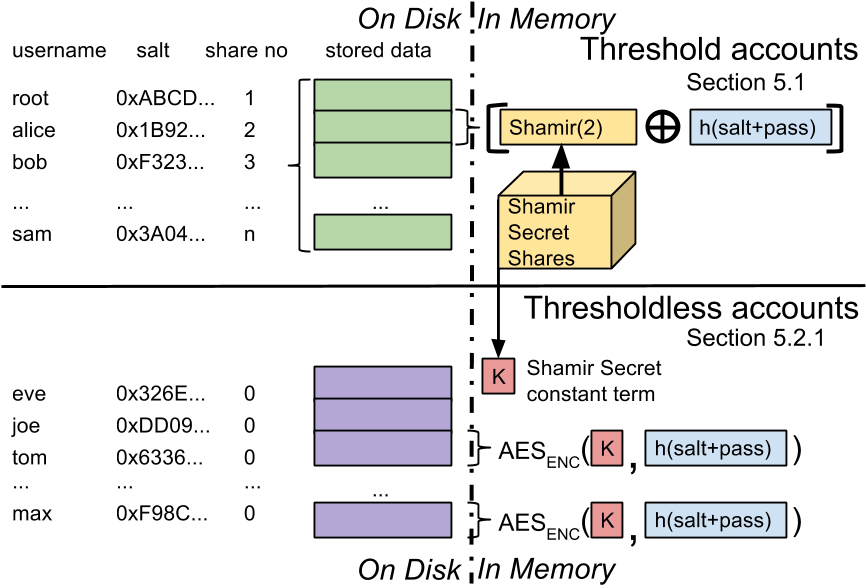
\includegraphics[width=\columnwidth]{figures/polypasswordhasheroverview.png}
\end{minipage}
\caption{The top portion of this figure demonstrates the data stored
by the basic PolyPasswordHasher algorithm.   The bottom portion shows how
thresholdless accounts have the salted hash of their password
encrypted by an AES key.   This AES key is stored as the secret for the 
threshold accounts and can only be recovered by the system if a threshold
of administrator passwords is known.}
\label{fig-polypasswordhasheroverview}
\end{figure}


\subsubsection{Checking A Password}

Assuming the server has enough valid passwords (and thus shares), the server 
can thus recover all shares.
The server computes the salted hash of the user's password and
XORs it with the last entry from the table (share XOR hash) to obtain 
the share.   If the share is valid, the password is correct.   The share will
consist of a set of $x$ values and $f(x)$ results.   To compute validity, 
one can evaluate $f(x)$ at the respective values and check to see if they
match.

Note that, a single account could optionally provide access 
to multiple shares.
To do this, there can be several entries with the same username that unlock 
using the same password, however each entry will have a different
salt and share number which leads to different stored data.   In this
case, the same password is hashed with different salt
and share numbers which effectively re-randomizes each component of
the stored data.

\subsubsection{Creating An Account}


As is shown in the top half of Figure~\ref{fig-polypasswordhasheroverview}, 
to add an account entry, one must have four items: username, salt, share
number, and stored data.   The server
randomly generates a salt, chooses an
unused share number, and uses the password's hash and share to
compute the shared data.   For example, if a user {\tt alice} needs an
account, the system will find an unused share number, such as 2 in the
above example.   Then the system computes a random salt, prepends
it to {\tt alice}'s password and computes the hash of this value.
This hash is XORed with the Shamir Secret Share's share number 2 and is stored
as the fourth field of the PolyPasswordHasher store.   The username, salt, share
number, and stored data are written to the PolyPasswordHasher store.


\subsubsection{Changing A Password}

Changing a password is a simple process for an unlocked store.  
Optionally, the procedure for account change may require validating the 
existing password first before allowing replacement.  The remaining steps 
required to change a password are nearly identical to account creation.  
The actual password change simply 
involves creating a new entry with the same username and sharenumber, but 
a different salt.  Since the salt and password have changed, the final
field will also change.   Once the new password entry is computed, it 
can replace the old one.   

If the PolyPasswordHasher database is also likely to be compromised, then it 
makes sense to additionally change the cryptosystem's secret information.
The reason is as follows.   Suppose an attacker compromises the password 
database repeatedly and knows the password for different accounts over a 
period of time.   From this information, the attacker may be able to recover 
enough shares from the
cryptosystem even if those accounts were not active at the same time.   To
combat this, one can easily change the cryptosystem's source of randomness
by computing a new random cryptosystem and XORing both the old and new 
shares with each stored data entry.   This effectively removes the prior
cryptosystem data while simultaneously adding randomness from the new
cryptosystem.   In this case, no user passwords are changed, so this
operation is not visible to the users in any way.


\subsubsection{Unlocking a PolyPasswordHasher Store}

To recover the random coefficients, the server takes a series of logins that 
have more than the threshold number of entries.   
%In fact, the server can (and should) check
%more than the threshold number of shares to validate the store is correctly
%unlocked.  
The server can either batch login requests and issue them all at once to
achieve this or simply wait for administrators with a sufficient threshold to 
attempt to login.   Then the password hashes are computed and the shares
are recovered.   Assuming that the provided information is valid, the 
cryptosystem will be able to use a technique like Lagrange interpolation to
recover all shares.

If more than the threshold number of shares is provided and some may be
invalid, individual user accounts (which may have 
incorrect logins) can be removed from the threshold to test their validity
so long as at least $k$ entries are validated.   %PolyPasswordHasher can leverage
%substantial prior work that detects and recovers from incorrect 
%shares~\cite{carpentieri1995perfect,Yang_compsac_02,devet2012optimally} in 
%threshold cryptosystems to find a valid set of entries.   
Furthermore, 
Section~\ref{sec-partial} describes an extension to partially validate 
passwords and discard a large percentage of incorrect values even before 
the threshold is reached.




\subsection{PolyPasswordHasher Extensions}
\label{sec-extensions}

There are three major limitations of PolyPasswordHasher as described in the previous
section.   
First, for some systems like Facebook or gmail, an attacker may control a
huge number of accounts.  In practice there are really two 
types of accounts: those that should count toward the threshold (likely 
administrators or power users) and those that should not.   This section
describes an extension to support ``thresholdless'' accounts that do not 
count toward the threshold.
Second, there is not a way to handle non-password authentication schemes
like biometrics, private key authentication, etc.   This section 
discusses how to integrate into existing mechanisms.   
Third, the system
must have a threshold of correct passwords before any can be authenticated.
This may cause logins to be delayed for an unacceptable time after a restart.
This section discusses an extension that leaks partial information about salted 
password hashes, but allows immediate authentication upon restart.   As a 
result, PolyPasswordHasher still provides an exponential security increase, but 
no longer must wait for account logins upon restart.




\subsubsection{Thresholdless Accounts}
\label{sec-thresholdless}

A desirable property is the ability to handle user accounts that should
not count toward the threshold.  For example, gmail and Facebook have 
a huge number of users that are untrusted and can create their accounts 
automatically.   None of these user accounts, no matter how many, should be
allowed to count toward the threshold for verifying other accounts.   

We will support accounts that should not count toward the threshold by
computing their salted hash and then encrypting this data with
a symmetric cryptographic cipher (AES).   If the server knows the AES key, 
it can clearly authenticate thresholdless users.
However, if the AES key is stored on
disk, an attacker that compromises the password file could compromise the
AES key too.   

To protect the AES key while stored on disk we will use a slightly modified
version of the PolyHashing store algorithm.   This store is identical to 
the main algorithm except
that the lowest order term (the constant term) of the polynomial represents 
a portion of the encryption key, as is shown in the bottom half of 
Figure~\ref{fig-polypasswordhasheroverview}.   (The key is stored in the same manner
as traditional Shamir Secret Sharing
where the constant term of the Polynomial encodes the secret.)
A party that knows the threshold of administrator passwords can XOR those
values to recover sufficient shares to reconstruct the polynomial (and thus
the key).  
By the properties of Shamir Secret Sharing, the key has information-theoretic 
privacy from an attacker unless they possess a threshold of account passwords.



Creation of a thresholdless account involves a similar series of steps to
other PolyPasswordHasher passwords.   As before the system obtains the 
salted hash for the password.   However, the salted cryptographic hash of 
the password is encrypted with AES instead of XORing it with a share.
To indicate this is a thresholdless account, the share field can 
be set to 0 to indicate that this is not a normal PolyPasswordHasher 
store.   (Note that the share 0 will not be used normally in Shamir secret
sharing.)   When the user attempts to login, if a large enough 
threshold of passwords has been entered, the AES key is available to decrypt 
the hash, allowing the user to  be authenticated.   However,
if the stored threshold data is disclosed, it is not useful to an attacker
unless they can recover the AES key by knowing a threshold of
administrator passwords.


If desired by an administrator, accounts can be switched between thresholdless
and threshold without user intervention.
In both the case of threshold and thresholdless accounts, a server with
a threshold of shares knows the information necessary to recover the salted 
secure hash.   This salted secure hash can then be re-encoded in the 
alternative manner and the new entry can be stored.

\subsubsection{Handling Alternative Authentication Mechanisms}

Passwords are not the only mechanism for logging into modern systems.   For
example, it is common for users to use a private key to login over {\tt
ssh}, biometric-based authentication holds substantial promise, 
smart cards are often used to hide user credentials, and single
sign-in systems like OAuth and OpenID are commonplace and provided by 
many major websites.   Any practical protection mechanism needs to operate
in conjunction with such techniques.

Handling non-password login for \emph{thresholdless} user accounts is trivial 
because
it requires no changes to the system.   Non-password login can be handled 
using the existing login mechanisms without any modification.
This is especially important for techniques like OAuth and OpenID which 
are almost certainly not going to be used to protect administrator accounts
(which count toward the threshold), but will be desirable to average users.

For administrator accounts or other accounts which are expected to contribute
to the threshold, one must devise other techniques.   Fortunately there is
a significant amount of prior work on secure remote authentication and
techniques for using this to hide 
secrets~\cite{deo1998authentication, yang1999password}.   This can be used to 
protect the Shamir Secret Share(s) for the account.
It is possible to view the authentication as decrypting information using a 
secret stored by a remote party (as in fact many such systems are implemented).
We can encrypt the Shamir Secret Share for the user with their key and then
check that the resulting $x$ and $f(x)$ are correct for the user.   

For example, suppose that an administrator has a private key that they use
to login (as is common with SSH private key authentication or smart card
based authentication).   Instead of
XORing the Shamir share with the salted hash of the password, it can
be encrypted with the user's public key.   When the administrator presents
their key to login, this key is used to decrypt the original share.   This
process can be repeated multiple times if the user has multiple shares.
 The share can then be used the same as any other share to 
unlock a PolyPasswordHasher data store.


For authentication of threshold account using other techniques such as 
biometrics, there has been prior work on deriving a private key from this 
(noisy) data~\cite{juels2006fuzzy}.   Once a key is derived from the biometric 
data, the scheme will function identically to the private key authentication 
scheme discussed above.




\subsubsection{Partial Verification}
\label{sec-partial}

When a PolyHashing store restarts, no values may be authenticated until a
threshold are provided.   If the time delay is not important and the rate
at which values are provided is rapid, this may not pose a problem.   However,
in many scenarios, this delay may prove burdensome.

This issue can be addressed with a technique called \emph{partial 
verification}.   Partial verification has the password database
leak partial information about the hash to allow verification before a threshold
is reached.   The core idea is similar for threshold accounts and 
thresholdless accounts, but for simplicity will be explained with threshold
accounts first.   If the Shamir Secret Share is chosen so that it is shorter
than the hash value, this will leak some bytes of the salted hash.
The `partial' hash that is leaked can be used for verification purposes.


\begin{figure}[t]
\center
% We need pdflatex with png images. Plain latex would fail here.
% So, we conditionally include this so we can still build with latex,
% just without this image.
%\begin{minipage}[b]{\linewidth}
\includegraphics[width=1.05\columnwidth]{figures/partialverification.png}
%\end{minipage}
\caption{This figure shows validation using partial verification.
A portion of suffix of the salted hash is stored on disk.  This
allows verification of accounts before a threshold of correct passwords is
provided.
}
\label{fig-partialverification}
\end{figure}

For example, suppose there is a 32 byte salted hash and a 30 byte 
secret (Figure~\ref{fig-partialverification}).   The secret will XOR with
the first 30 bytes, effectively obscuring them.   However, the remaining
2 bytes will consist of the suffix of the salted hash.   When the
system restarts, accounts can be validated using the last 2 bytes of the
hash.   Once sufficient accounts have logged in, the full
hash can be recovered and account authorizations can be 
performed using the full hash as was described in the 
previous section.

Thresholdless accounts can also be validated before a threshold is reached
if partial validation is used.   The technique is similar to threshold 
accounts, where a portion of the suffix of the hash replaces
some of the encrypted hash on disk.   Validation can be 
performed with the suffix until a threshold of correct passwords are provided
and the Shamir Secret Store (and thus the AES key) are recovered.

Increasing the length of the hash which is leaked has a negative 
effect on the resulting data store security.
First of all, suppose that $l$ bits are leaked with via the hash.
This allows an attacker that compromises the password hash database to 
discard $2^l$ possibilities from the password search space.   Thus
if there is a threshold of $k$ and each password has $n$ bits of entropy, 
the attacker can make $k$ passes of cost $2^n$ to remove all but $2^{n-l}$
passwords.   Following this, the attacker will then need to simultaneously
guess from the remaining passwords which will cost an additional $2^{k*(n-l)}$
to crack the store.   (Section~\ref{sec-feasibility} discusses the practical
impact this has on password security.)

However, a small hash also has a negative ramification that
incorrect passwords could log in before a threshold is reached.   In fact,
the probability of a random password working is $\frac{1}{2}^l$.   Rate
limiting the rate of password attempts can mitigate the risk from an attacker
that does not know the salt.   However, if an attacker has stolen the password 
database, they can quickly compute a value that will be correctly verified 
upon restart.  However, once a threshold of passwords is provided,
PolyPasswordHasher knows the full hash and can detect any such
malicious logins.   Much like other decoy schemes~\cite{juels2013honeywords,
Kontaxis_CCS_2013}, partial verification allow incorrect logins but
later detects this occurrence and provides strong evidence that the password
database was leaked.

\eat{
The length of the leaked information need not be the same for every 
account.   There is no reason why the threshold and thresholdless accounts
need to have the same length of leaked information.   In fact, every 
thresholdless account could have a unique quantity of leaked information,
perhaps to take into account entropy in the password.   For threshold
accounts, a variable amount of leaked information could be appended to each
share.   Since the shares hide the secret, leaking hash
information effectively leaks some parts of the shares to the attacker.
We will study the security implications of leaking variable portions of 
threshold accounts in future work.

}







\section{Discussion}
\label{sec-expecteduse}

This section discusses strengths, limitations, and expected uses of 
PolyPasswordHasher as compared to other techniques.


{\bf How does PolyPasswordHasher compare to having an administrator enter a key
at boot time to unencrypt the password database in memory?}

With the administrator entering a key, the system cannot validate passwords 
upon startup until an administrator intervenes.  With partial verification, 
PolyPasswordHasher can process user authentications immediately.   Furthermore, 
if the administrators enter a key, all system administrators would likely 
share this key to be able to quickly act to restart the system.   From 
a security design standpoint, it is considered bad practice to share
passwords.  With 
PolyPasswordHasher different administrators do not need to share a password or key.
Each administrator may have their own password allowing access control to 
happen naturally as administrators join and leave the organization.


{\bf Why not store a key to decrypt the password database in hardware instead?}

Storing a key in trusted hardware (such as a USB 
dongle~\cite{passwordhardwaredongle}) has security benefits,
but also has significant deployment challenges.  
%The software must be rewritten to interface with that 
%manufacturer's secure token.   
If the hardware stops working, the protected data is 
likely to be irrevocably lost.  %Furthermore, 
To have backup servers, it is essential to have identical 
duplicate copies of the secure token.   This complicates use in scenarios 
like cloud computing or even just a standard master / slave deployment.
On the other hand, PolyPasswordHasher is entirely software based and a backup system
can be brought online in the same way that a normal server boots.



{\bf How does an attacker that can read arbitrary memory on the 
authentication server impact PolyPasswordHasher?}

If an attacker can read arbitrary memory on a running server where the 
threshold of authentications has been met, the attacker can recover
the Shamir Secret Store.   This allows the attacker to recover the 
hashes for each password.   An attacker could then crack passwords
individually in the standard way.    While these are not the majority of
disclosed database compromises~\cite{passwordresearchblog,miranteTR13}, 
neither PolyPasswordHasher nor techniques like hardware key storage 
are significantly helpful in this situation.
%protect against situations where the attacker has administrator access on a 
%running authentication system.

Furthermore, new processor extensions such as Intel 
SGX~\cite{mckeen2013innovative} expressly provide protections to select 
portions of user space code so that even a root user, hypervisor, or the 
operating system kernel cannot read it.   Servers running PolyPasswordHasher can 
leverage these extensions to protect the Shamir Secret Store.

However, if an attacker can read
arbitrary memory, the attacker can gain access to plaintext passwords
as they are provided by clients.    This is because typically the client
provides the server with the password, which the
server then combines with the salt to get the hash.  
So without changes to the client software, any server-side
password storage technique will leak plain-text passwords to an attacker
that can read arbitrary memory on a running server.



{\bf How does PolyPasswordHasher change how users interact with existing password authentication systems?}

Using PolyPasswordHasher results in very minor changes to existing password
authentication systems.   
%The only user perceptible difference is when 
%the system is restarted, authentication attempts will be delayed or 
%declined until the threshold is reached.   
%
The client tools for password authentication do not change in any way.   In 
fact, because PolyPasswordHasher only impacts password storage, it is invisible to 
clients.   %A user cannot tell if PolyPasswordHasher is being used, much like it is 
%not possible for a user to tell if a server stores a password using a salted 
%secure hash or in plaintext.
For the administrator's toolchain, the only change is that 
when an account is created, the administrator can specify if the account counts
toward the threshold or not.
%Note that in many cases, such as cloud services, the 
%separation for threshold and thresholdless accounts is clear.   For example, a 
%web service may choose to have a command line interface used by administrators
%to create accounts with a threshold, while the web interface will only
%create thresholdless accounts.

{\bf How does using PolyPasswordHasher integrate with existing password storage 
formats?}

The file format for password storage is similar to existing systems.
For systems which use a database, one can simply insert the share number
as a new column in the table and change the authentication logic to include
PolyPasswordHasher.   

However, 
many servers (such as Linux, Mac and BSD) use the {\tt /etc/shadow} or 
{\tt /etc/master.password} file 
colon delineated formats.
%by `:') such as the username, password expiry date, last date the password was 
%changed, and a single `password' field.
The `password' field contains both the salt and hash but these
different portions of the field are not 
delineated.  
%Instead the storage and verification code knows which 
%bytes of the `password' field are used for each task.   
For PolyPasswordHasher, one can also add the share number at a known byte location
within the `password' field (such as the beginning or end), making this
variable length, opaque string one byte longer.
%We do not anticipate issues with this since the `password' field and length
%are opaque.  (In fact administrators commonly change the length and content of
%the `password' field manually.)   Other fields are separated from the password
%field using `:' as a delimeter and so will not be impacted.


{\bf If there is a single administrator, is PolyPasswordHasher useful?}

There is value in PolyPasswordHasher whenever there are multiple
accounts, even if only one is an administrator.   If an attacker steals the
password file, but does not know the password for the administrator account, 
the attacker cannot crack other user accounts.   
Assuming that the attacker does not know the administrator password
from other sources, such as its use on multiple sites, the 
attacker cannot crack a thresholdless password without cracking 
the administrator password.


{\bf What threshold values are likely to be used?}

%It is logical to assume that most policies for login will request that
Ignoring partial verification,
$k$ of $n$ administrators (or power users) must login to unlock the
PolyPasswordHasher store.   The value of $n$ is largely irrelevant
except it must be smaller than the field size since there are only $n-1$ 
Shamir Secret shares.   (Note $n$ only includes accounts that should count
against the threshold.)
%
%The primary value that matters is $k$, the threshold setting.   
%The threshold value $k$ is the number of individuals 
%that must enter their password before unlocking a data store.   
%A very large value may impact the availability of the system since logins 
%cannot be processed until the threshold is reached.   
We believe that most organizations will have a small 
value for $k$, such as $1$ to $5$.   As our results later show, 
when coupled with non-trivial passwords, even a small value of $k$ 
increases password strength immensely.



{\bf When is PolyPasswordHasher most (and least) valuable?}

When only a single user account exists, such as on a smartphone, 
there is no benefit to using PolyPasswordHasher on the local device.   However, 
essentially all devices are networked and interact with servers.   Web and 
cloud services benefit from PolyPasswordHasher as do any devices that support
multiple user logins.   
Services that manage logins from multiple parties, substantially benefit from
PolyPasswordHasher.     This is because PolyPasswordHasher makes 
a password file compromise only impactful if a threshold of administrator
passwords are already known.   %We believe that any organization that has 
%passwords from multiple users and wants to protect those
%passwords (which should be a universal goal) should deploy PolyPasswordHasher.


{\bf What happens if so many threshold users forget their passwords that a
threshold cannot be reached?}

If there are not enough known threshold users, all password data in the
password file is useless.   However, this does not mean that the device is
unusable.   If used, partial verification will still allow users to log in.   
However, it will not be possible to create new accounts since Shamir
Secret Shares cannot be generated and the AES key protecting the thresholdless
accounts is not known.  Furthermore, mechanisms like root password recovery 
through
the console will still work, allowing any data on the system to be accessed.




%{\bf Why might PolyPasswordHasher be adopted when existing schemes are infrequently 
%used to protect passwords?}
%
%A huge advantage of PolyPasswordHasher is that it is a software-only solution that
%requires no additional hardware or setup.  The only change is in the 
%authentication software.    Furthermore the change is not burdensome (or even
%visibile) to end users.   We believe the power of simply allowing an 
%administrator to improve security through a simple software action (like
%{\tt apt-get install polypasswordhasher}) could substantially increase adoption.



{\bf What happens if users choose extremely weak passwords like 123456, 
letmein, and password?}

Ignoring partial verification for the moment, 
if extremely weak passwords are used for a threshold of threshold accounts 
(like administrators), PolyPasswordHasher will not provide strong protection.   If
there are only a few bits of entropy in the password, while exponentially
larger, the search space will still be small.   It is thus critical that
the administrators choose strong passwords.   However,
if a thresholdless account uses a weak password, the attacker must first
crack a threshold of accounts, thus providing strong protection.

If partial verification is used, then some bytes of the password's 
hash are leaked.   If an extremely weak password is used, this
will be effectively leaked to the attacker.   One should think of partial
verification as reducing the password strength via the number of leaked
bits.   Thus a password with fewer bits of entropy than the partial 
verification length, can be cracked as though it is protected using today's
best practices.


Independent of all of this, extremely weak passwords are susceptable to 
guessing by an external party (without database access) and as best practices
sites should block them from use~\cite{bancommonpasswords}.






\section{Implementation}
\label{sec-implementation}


Our reference implementation for PolyPasswordHasher is available with an MIT license 
at \showurlx.  It utilizes
a 16 byte salt, with SHA256 to compute password hashes.   The Shamir
Secret Sharing routines
utilize GF256 as the underlying field (encoding each byte as a separate
share).   %The implementation of Shamir Secret Sharing was written while
%referencing the open source Python {\tt tss} implementation, but was 
%essentially rewritten to handle the interfaces needed by PolyPasswordHasher.   
The full code base for PolyPasswordHasher is 203 lines of Python code and
223 lines of C code\footnote{
All line of code counts are according to SLOCcount~\cite{wheeler-sloccount}}.   
PolyPasswordHasher uses Python's standard hashlib for SHA256 and the PyCrypto
implementation of AES.
The GF256 operations, Lagrange interpolation, and polynomial math code
are written in C for performance reasons.   All other code is written in 
Python.  The main code for PolyPasswordHasher, which handles account
creation, accessing a persisted store, writing a store to disk,
checking passwords, and similar operations, is 87 lines of Python code.
Adding support for thresholdless accounts involved adding 20 lines of Python
code.   Partial verification added 13 lines of Python code.
The remaining Python is wrapper code for the C-based 
Shamir Secret Sharing implementation.

%\url{https://polypasswordhasher.poly.edu/}.   
%We release the code as open source 
%under an MIT license.





\section{Evaluation}
\label{sec-evaluation}

\begin{figure}[t]
%\begin{minipage}[b]{.45\linewidth}
    \includegraphics[width=.75\columnwidth, angle=270]{resultdata/onebigtimegraph.eps}
	\caption{Time for PolyPasswordHasher operations.  The plots for thresholdless
creation and verification overlap as do the plots for the threshold versions
of each action.}
	\label{fig:time_basic_operations}  
\end{figure}
%\end{minipage}
%\hspace{.06\linewidth}
%\begin{minipage}[b]{.45\linewidth}
%    \includegraphics[width=.75\textwidth, angle=270]{resultdata/onebigperformancegraph.eps}
%	\caption{Performance (operations per second) for PolyPasswordHasher operations.  }
%	\label{fig:performance_basic_operations}  
%\end{minipage}
%\end{figure*}
This section describes a performance evaluation of our prototype of 
PolyPasswordHasher.   
To understand the performance of PolyPasswordHasher,
we performed a series of microbenchmarks on an early-2011 MacBook Pro with 
4GB of RAM, a 2.3 GHz Intel Core i5 processor.  


%\begin{figure}[t]
%    \includegraphics[width=0.3\textwidth,angle=270]{resultdata/onebigtimegraph}
%	\caption{Time for basic PolyPasswordHasher operations.  }
%	\label{fig:time_basic_operations}  
%\end{figure}
%
%\begin{figure}[t]
%    \includegraphics[width=0.3\textwidth,angle=270]{resultdata/onebigperformancegraph}
%	\caption{Performance (users impacted by an operation per second) for basic PolyPasswordHasher operations.  }
%	\label{fig:performance_basic_operations}  
%\end{figure}

All operations are the mean verification time across 100 runs and
are performed with the password file already present in
memory.  
For benchmarking purposes, each action is performed sequentially despite being 
embarrassingly parallelizable.


\subsection{Performance Of A PolyPasswordHasher Store}

%To evaluate the performance implications of PolyPasswordHasher, we varied the 
%threshold.   While we do not believe that
%there will be many (if any) practical situations where the threshold would be 
%set to a value larger than ten.
%However, for completeness, we show the result of varying the threshold
%across a broader range of possible values.   
Figure~\ref{fig:time_basic_operations} shows the time taken by
different operations (discussed below).  Unless noted below,
the time of the operations does not depend on other factors such as the 
number of accounts in the password database.




{\bf Account Verification.}
The mean verification time of a threshold account
varies from 57$\mu$s to 163$\mu$s depending on the
threshold.  With a threshold of 8, this allows the verification of 
more than 16K user accounts per second.

Thresholdless accounts are verified in a time that is independent
of the threshold size because it merely computes    
a salted hash and performs an AES encryption operation.
Verifying
a thresholdless account takes about 29$\mu$s, allowing
about 35K such actions to be performed each second.   
In comparison, the current
best practice of generating the SHA256 hash of a known salt is a little over
3$\mu$s on the same hardware, which allows hundreds of thousands of
account authentications per second.   
%Note if there were a case where the account 
%validation software needed to process more than 35K account authorization
%attempts per second, the process is embarrassingly parallelizable.



{\bf Account Creation / Password Change.}
The account creation time is similar to that of password verification.
Depending on the threshold, the average verification time 
varies from 77$\mu$s to 190$\mu$s.  
A store with a threshold of 8 can create more than 12K 
accounts per second.   Given there are a maximum of 255 threshold accounts
that can be created (at least with a PolyPasswordHasher implementation that uses
GF256), this clearly is not a performance concern.


Much like account verification, thresholdless accounts can be created in 
time that is independent of the threshold.   
A thresholdless account creation takes about 25$\mu$s.   As a result, 
about 40K thresholdless accounts can be created each second.   This is
similar to the time it takes to generate a salted SHA256 hash for a 
provided password (16$\mu$s). 

Note that changing the password requires that PolyPasswordHasher performs the same
operation as account creation (potentially along 
with authentication of the old password).


{\bf Initializing a Store.}
The time to create a store varies depending on the threshold.   This
cost is dominated by generating cryptographically-suitable random
numbers.   By varying the threshold, the creation time varies from 
380$\mu$s to 1.13ms.   This operation is only performed when a 
new password file is created.

{\bf Unlocking a PolyPasswordHasher Store.}
When the server restarts, the
random coefficients are computed from the set of provided shares with
full interpolation.   The time needed varies 
between 202$\mu$s and 2.87s as the threshold changes since
the number of polynomials changes as the store size grows.
Note that small thresholds are very fast, with a store with a threshold of 8
being unlocked in 617$\mu$s.

This is fast enough that if some passwords are incorrectly entered, 
PolyPasswordHasher can (na\"ively) detect them.   For example, suppose that
a threshold of 10 is used and that 14 passwords are provided and only
10 of them are correct.   All possible combinations of 10 passwords can be
checked by PolyPasswordHasher in 618ms.
Partial verification will also discard most passwords that are entered 
incorrectly to prevent them from being used to attempt to unlock the 
password store.
% If there is a huge threshold with a large number of
%candidate logins and passwords, it would also
%be possible to apply more advanced techniques for detecting incorrect
%shares~\cite{carpentieri1995perfect,Yang_compsac_02,devet2012optimally}.


%Furthermore, this process needs only to be performed when the 
%system is restarted.  


\subsection{Memory and Storage Costs of PolyPasswordHasher}


\begin{table}[t]
{\scriptsize
\begin{tabular}{|l|l|l|l|}
\hline
Password & Original & Salted, Hashed & PolyPasswordHasher \\
Source & Disk Space & Disk Space & Disk Space\\
\hline
\hline
eHarmony* & 51.6MB & 100MB & 102MB \\
\hline
Formspring* & 27.3MB & 34.8MB & 35.2MB \\
\hline
Gawker & 75.2MB & 119MB & 120MB \\
\hline
LinkedIn* & 252MB & 424MB & 430MB \\
\hline
Sony & 2.98MB & 4.95MB & 5.00MB  \\
\hline
Yahoo & 17.8MB & 35.0MB & 35.4MB \\
\hline
\end{tabular}
}
\caption{Disk space to store password data from different account disclosures.
Entries with a * indicate only the password hash portion of the database
was leaked.   Other breaches include usernames and similar data.  }
	\label{tab:extrahashcost}  
\end{table}



%\begin{table}[t]
%{\scriptsize
%\begin{tabular}{|l|l|l|}
%\hline
%Storage Mechanism & Disk per entry & Total memory cost\\
%\hline
%\hline
%Salted Secure Hash & 48 bytes & N/A (stored on disk) \\
%\hline
%Threshold & 49 bytes & $k*32$ bytes (likely $<1$KB) \\
%\hline
%Thresholdless (separate file) & 48 bytes & N/A (included in threshold) \\
%\hline
%Thresholdless (same file) & 49 bytes & N/A (included in threshold) \\
%\hline
%\end{tabular}
%}
%\caption{Cost to store the password hash database for PolyPasswordHasher and 
%conventional salted hash techniques in terms of memory and disk space.
%A 16 byte salt and 32 byte hash is assumed for all schemes.}
%	\label{tab:extracost}  
%\end{table}

Storing passwords with PolyPasswordHasher requires additional information be stored
for each account.   Namely, for each account, since each share is a value
in GF256, there must be a one byte share number stored for each account.   
This represents an additional 1 byte of storage space for each account in 
addition to the cost of current hash techniques.   This
has a minimal impact on the disk space needed to store production
password databases (Table~\ref{tab:extrahashcost}).   If the thresholdless 
accounts are stored in a separate file or are
otherwise distinguished, then only threshold accounts require the extra
byte of storage.   This will result in a cost for those accounts that is
identical to the salted, hashed scheme.

In addition, any account that has 
multiple entries (to count multiple times toward the threshold), requires an 
additional salt (16 bytes), hash (32 bytes), and share number (1 byte)
for every entry after the first.
Since there are at most 255 Shamir secret shares in GF256, this can be treated 
as a fixed cost of a few kilobytes.
%We do not believe the additional storage 
%cost will prove a burden in any practical scenario.

There is additional memory cost because the server must cache
the polynomial coefficients for a store.   The total
size of this data is the threshold value multiplied by the hash length.
Thus, the in-memory threshold data is likely to be under a 
kilobyte in practice.% (Table~\ref{tab:extracost}).   This is likely to be smaller than the (also minimal)
%memory space needed to store the additional code for PolyPasswordHasher.
When thresholdless accounts are used, the AES key used is the 
constant term 
of the polynomial coefficients and so does not incur additional cost.
The use of partial verification has essentially no impact on the storage or 
memory requirements.

%Note that if thresholdless accounts are used and stored in the same
%file as threshold accounts, the disk costs
%are the same for both types of accounts (Table~\ref{tab:extracost}).   
%In order to indicate an account is thresholdless while using the same
%password database, the share number can be 
%set to 0 (an invalid share in traditional Shamir Secret Sharing).
%%There is the same memory and disk storage costs for each account regardless
%%of whether or not it counts toward the threshold.
%This indicates the account is thresholdless while permitting storage
%in the same file.




%\subsection{Thresholdless Accounts}
%
%\cappos{AES can compute about 400K 256 byte decryptions per second on my 
%laptop.   This is much faster than even SHA256, so should be much faster than
%accounts with a threshold.}


\subsection{Feasibility Of Cracking Passwords}
\label{sec-feasibility}

\begin{figure}[t]
\hspace{-4mm}
\includegraphics[width=.36\textwidth, angle=270]{resultdata/plotcrack.eps}
	\caption{Time to crack a password store given 1 billion attempts
per second.   The k=1 case for PolyPasswordHasher is the same as the
legacy salted hash scheme.   The partial verification values show 
how leaking 2 bytes impacts cracking time.   A threshold of 3 without partial 
verification falls well outside the axis of the graph.}
	\label{fig:cracktime}  
\end{figure}

%Assuming a threshold of accounts is not known, cracking passwords takes 
%exponentially more time with PolyPasswordHasher than standard hash
%schemes.   The reason is that an attacker must simultaneously attempt to
%crack the threshold number of passwords at once.
%An attacker must attempt to determine the random coefficients that are 
%protected by Shamir Secret Sharing before validating passwords.   This means 
%the attacker must know enough passwords to have at least the 
%threshold number of passwords.
%If an attacker needs to guess $p$ passwords, where each password has $V$ 
%possible values, the attacker is choosing values from $V^p$ possible guesses.   
%Solutions that involve slower hash functions or multiple hash iterations 
%result in only a linear increase in attack time and verification time.
%Since passwords must be correctly guessed simultaneously with PolyPasswordHasher, 
%PolyPasswordHasher results in an \emph{exponential} increase in attack time.

{\bf General Analysis.}
Even when an attacker needs to guess only a few passwords, in many cases 
PolyPasswordHasher's \emph{exponential increase} in guessing time ($O(V^p)$ instead 
of $O(pV)$) makes guessing computationally infeasible 
(Figure~\ref{fig:cracktime}).   For example, suppose 
an attacker wants to guess three passwords that they know are each comprised 
of 6 randomly chosen characters\footnote{These passwords
are extremely weak and we do not advocate their use.   This 
example is used to illustrate the strength of PolyPasswordHasher even with 
weak passwords.}.  Recent results 
have shown that a GPU can compute on the order of a billion password hashes a 
second~\cite{ElcomSoftGPUCracking, zonenberg2009distributed}, allowing the 
attacker to search the key space for all three passwords in under an hour.
Thus the current state of the art provides little protection in this case.

In the case of PolyPasswordHasher, the attacker must \emph{simultaneously}
guess all three passwords.   This means the attacker needs to guess from 
$3.97 \times {10^{35}}$ values.   This is roughly 23 orders of magnitude more effort.
When PolyPasswordHasher is used with the same passwords and the GPU 
accelerated technique, searching the key space would take $1.25 \times 10^{19}$
CPU years (does not fit on the axis of Figure~\ref{fig:cracktime}).   To put 
this number into context,
ignoring smartphones there are about 900 million computers on the 
planet~\cite{computersexisting}.   The estimated age of the universe is 
$(1.3798 \pm 0.0037) \times 10^{10}$~\cite{universeage}.   The time needed to crack 
three random 6 character passwords protected
by PolyPasswordHasher is more CPU time than would be provided by every computer 
on the planet working nonstop for the estimated age of the universe!

Even a threshold of two is substantially stronger than existing
best practices.   Searching the key space would require over 17 million CPU 
years of effort.

%If partial verification is used, this effectively allows accounts to be
%compromised by reducing the password entropy by the number of bits
%leaked.   However, assuming the remaining number of bits is positive, the
%passwords must then be simultaneously cracked.   In essence the attacker
%precomputes a candidate list of likely allowed passwords based upon the leaked
%data and can then try all combinations of those passwords.

{\bf Partial verification.}
Partial verification allows an attacker to first reduce the search space for
a specific account by eliminating accounts that do not match the leaked bits.
If the attacker knows the password pattern, the attacker can first 
precompute all passwords that match that pattern and hash.   This requires
the same amount of effort ($k*2^n$) as cracking passwords when stored with 
traditional best practices.   If the attacker has sufficient space to
store these passwords, the attacker then may use combinations of
these precomputed passwords to try to unlock the store.  This allows
the attacker to search the space for the Shamir Secret Store in $2^{k*n-l}$ 
guesses. 
Each byte used for partial verification effectively
reduces the strength of a random password by approximately 1.22 characters.
However, the time needed to unlock the Shamir Secret Share still represents
an exponential increase and dominates the overall cost.

For example, if 2 bytes are leaked for 6 random character
passwords (Figure~\ref{fig:cracktime}), the attacker will need to do
735 trillion operations for each of the
three passwords and then $1.41 \times 10^{21}$ operations to crack the password
store.   With one billion operations per second, sweeping the search
space would still require 45 thousand CPU years (8 orders of magnitude
more time than salting and hashing).
%password strength if used, even with partial verification PolyPasswordHasher still
%represents a huge benefit over only salting and hashing.






{\bf Case Study.}
To explore how these results hold for real passwords, we performed an
experiment using the password data dumped from the Sony account breaches
\cite{sonyhack}.   Of the leaked passwords known to the authors
(Table~\ref{tab:extrahashcost}), this is the only data set which 
explicitly lists which accounts are administrator accounts versus normal users.

In the database dump, there is password data for both outside
user accounts as well as accounts have administrator access.   (There is
also a database with testing accounts which we ignore.)
The four administrator accounts have passwords with the estimated
entropy in bits~\cite{passwordstrength}:
password@1 (5.322 bits), %Annelies (17.653 bits), 
welkom@1 (26.553 bits),
waderobsen (30.618 bits), %foto4U2 (31.186 bits), fietspomp@1 (42.139 bits),
and itsafullcyrcle (44.011 bits).   
Given a rate of checking a billion password hashes a second, the first 
three passwords can all be cracked in two seconds.   The
remaining password (and thus every administrator password) could be
cracked in under 5 hours.
%Using John the Ripper, version 1.7.9-jumbo-7 built for macosx-x86-64, with
%the default settings on a early 2011 era Macbook Pro, allowed the passwords
%to be cracked in .
%In comparison, 948K of the 6.5M unique LinkedIn passwords were cracked within
%1 hour of computation on the same system / program.

If PolyPasswordHasher were protecting these passwords, the ability to crack the
passwords depends on the threshold.   The effective password strength is 
that of the weakest passwords combined, times the probability of selecting
those accounts in that order.  
A threshold of 3 will have an effective entropy of 67.078 bits,
which will take nearly 5000 years to crack at 1 billion guesses a second. 

With a threshold of 2, the effective entropy
is 35.459 bits, which can be cracked in under a minute.   
However, if all administrators had chosen a password
as strong as the password waderobsen (which is considered a weak
password by best practices~\cite{passwordlength}), then the password would 
have had an effective 
entropy of 64.820 bits, which will take more than a thousand CPU years to crack
at 1 billion guesses per second.   This underscores that administrators
still should not choose immensely poor passwords like password@1.   
Independent of password storage, avoiding trivially guessable passwords 
is essential to prevent remote brute-force password cracking.

The thresholdless user passwords (many of which are extremely poor) 
cannot be cracked until a threshold of administrator passwords are 
compromised.  This means that even if only administrators can be convinced to 
use strong passwords, PolyPasswordHasher provides substantial security benefits.





\eat{
% I like this, but it isn't really true given hashing validation of shares.
When strong passwords are used, the problem becomes even more intractable.   
In fact, with sufficiently strong passwords, it can be impossible to know that
one has correctly guessed the password.   For example, assume the attacker
knows one fewer than the threshold number of passwords and must guess only one 
other to know the random coefficients.   If the password hash and length is 
such that any possible hash value can be generated and all are equally likely 
(intended properties of hashing schemes), then all hashes are equally
likely.  This means in the extreme case where the password length is such that 
all hashes can be generated and all are equally likely, PolyPasswordHasher's use of 
Shamir Secret Sharing provides information-theoretic protection.
}


\section{Related Work} \label{sec-related}

%\cappos{ cite: \url{http://cs.gmu.edu/~csnow/library/unix/Klein_passwd.pdf} 
%and lots of other things}

%\cappos{A nice survey paper with related work details~\cite{tsai2006password}.}
There has been extensive work on password security stretching back many
years~\cite{morris1979password,klein1990foiling, florencio2007large}.   
Password database disclosure is a problem that, if anything, seems to be
more prevalent as time goes on~\cite{clair2006password,miranteTR13,passwordresearchblog}.
Password security has been the focus of much study with many promising 
solutions solving different portions of the problem~\cite{tsai2006password}.

Our work on PolyPasswordHasher is unique in that is the first password database
protection scheme that:
\begin{enumerate}
\item assumes the attacker can read all persistent storage,
\item requires only a software change on the server,
\item and requires exponentially more time for the attacker to crack passwords.
\end{enumerate}

PolyPasswordHasher can be deployed with minimal server changes and without modifying 
clients at all.   

{\bf Multi-server Password Authentication.}
There are a wide variety of authentication schemes that use multiple servers
to store password data~\cite{Chai20071046,bagherzandi2011password, katz2005two}.
The assumption is that the attacker cannot compromise a threshold of
the servers.  In contrast, PolyPasswordHasher uses a single server but uses
a threshold system to hide information that can only be unlocked
with a threshold of correct user passwords.

{\bf Decoys.}
Recently, researchers have suggested multiple techniques that use a set of 
extra password entries~\cite{Kontaxis_CCS_2013, juels2013honeywords}.  For 
example, the Honeywords~\cite{juels2013honeywords}
system uses a separate server holds information about which password entry is 
correct.   If an 
attacker obtains the password database then they do not know which password 
entry is correct.   Entering a password which matches the hash of a 
different password entry will trigger an alarm which notifies the 
administrator of a password hash file breach.   However, for this 
to work, there must be a separate, secure server which authenticates 
the index of that entry in the file (a one byte value).   
The real value of HoneyWords is that it can also operate when that server is
offline and / or check passwords at a later time to detect breaches later.
%If it is 
%possible to build such a system, it is not clear why that server 
%cannot simply securely store and check the password hash (a fixed 
%size value of about 32 bytes).  
PolyPasswordHasher utilizes ideas from these works in constructing the partial
verification technique discussed in Section~\ref{sec-partial}.

{\bf Key Stretching.}
One way to mitigate the effectiveness of password hash cracking is to
use techniques for key stretching~\cite{kelsey1998secure}.   This involves
performing multiple rounds of cryptographic operations to validate a key.
This effectively slows down both the attacker's cracking of passwords and the
user's authentication by the same factor.   In contrast, PolyPasswordHasher results 
in an exponential increase in the amount of time needed by requiring multiple
passwords to be simultaneously guessed.  Key stretching is orthogonal
to PolyPasswordHasher and could be trivially used in conjunction.
%that knows a threshold of correct account authentications.


%{\bf Hardware-based Password Database Encryption.}
%Several companies use password database protections that center
%around storage of keys or passwords in hardware, such as through a USB dongle.
%Hardware based solutions are fundamentally more 
%secure than PolyPasswordHasher since even if an attacker has access to all memory,
%the password database is not at risk.   
%Unfortunately, these systems are not widely deployed.
%One issue they face is that each device presents its own interface for password
%storage and decryption.   A company that wants to deploy a solution must 
%provide new authentication code for the specific device and also purchase
%the devices.   
%If the hardware token stops workting, the data may be irrevocably lost.
%If the server storing a device is damaged or crashes, it 
%is not possible to bring up a backup using the same authentication 
%database.  On the other hand, PolyPasswordHasher is a purely software-based solution.
%This not only makes it easier to deploy, but also means that a backup can be 
%brought online in the same way that the normal server boots.   As a result
%PolyPasswordHasher is much easier to deploy and manage in distributed computing
%environments such as in cloud computing.

%\cappos{Read over and add cites.}

{\bf Bounded Attacker.}
Di Crescenzo~\cite{di2006perfectly} proposed a scheme for protecting
password data when an attacker can only read a bounded amount of data from 
storage.   This works by an organization configuriing
network monitoring hardware and setting up a separate server to process 
authentication requests.
In the widely published password file compromises, the 
attackers were able to steal complete password file 
data~\cite{miranteTR13,passwordresearchblog}.   In contrast, 
PolyPasswordHasher requires no network changes or monitoring and works even when an 
attacker has complete access to stored information, such as a disk backup.

Prior work by Gwoboa~\cite{gwoboa1995password} hides passwords using
a trapdoor function (public key cryptography) and techniques from threshold
cryptography.   It can authenticate users with two hidden pieces of 
information, a user ID (likely not the user name for security reasons) and 
the password.   However, a major concern of the scheme is how the private
key is stored on the server.   The authors propose splitting it amongst 
multiple systems and using threshold cryptography.   Clearly if all 
persisted data is known, this key (and thus all passwords) are at risk.
In PolyPasswordHasher, as long as a threshold of passwords are not known, all 
persisted data can be stolen by an attacker without compromising user 
passwords.


{\bf Biometrics.}
Biometric authentication has substantial promise for secure
authentication~\cite{atallah2005secure, snelick2005large, tuyls2004capacity, 
boyen2005secure, erkin2009privacy, kerschbaum2004private, osadchy2010scifi,
monrose2001cryptographic, sae2012biometric}.
There has been a substantial amount of work on how to store and authenticate 
users with this information.   Like PolyPasswordHasher, some of these systems 
use a threshold of information to validate and authenticate users, in part
to deal with noisy biometric data~\cite{juels2006fuzzy, ballard2008practical}.  
While users must still remember a password to use PolyPasswordHasher, it does not 
require client-side hardware.

Prior work uses keystroke dynamics to change stored password 
data~\cite{monrose2000keystroke}.  This technique relies on reading timing 
information from when the user types their password into a site.   This 
provides promising protections, but requires changes to the client and server 
to correctly operate.   In comparison, PolyPasswordHasher protects password
hash information with no change to the client and minimal server changes.

{\bf Authentication Using Tokens or Smart Cards.}
Much authentication has looked at authentication in the context of
banking~\cite{deo1998authentication, yeh2010two}, health 
services~\cite{ahn2002towards},
or a more general context~\cite{chien2002efficient, yang1999password}.   These 
systems are
extremely effective and are widely used for banking and protecting access
to classified systems.   Unfortunately, these devices incur a per-user 
cost and thus are not often used in contexts where the user and server have
no prior commercial or authentication relationship.   PolyPasswordHasher can 
be applied to webmail systems and social networks where this relationship
does not exist a priori.

{\bf Two-Factor Authentication.}
The use of two-factor authentication~\cite{di2005two} is provided by some 
popular services (typically through a user's smartphone).   The use of 
two-factor authentication does not
change PolyPasswordHasher's use in any way.   Users can easily get the best of both
protections by a simultaneous deployment of each technology.



{\bf Multiparty Computational Authentication.}
There are a variety of schemes that perform secure, remote authentication using
computation by the client and server on legacy hardware~\cite{wu1998secure,
Lomas_SOSP_89, chien2001modified, jan1998paramita, gong1995optimal, 
camenisch2010credential, brainard2003nightingale,
katz2001efficient, katz2003forward, gong1993protecting}.  These schemes have 
significant positive aspects such as (in some cases) requiring an attacker to 
be online to validate communications.   However, they require multiparty 
protocols which require changes on clients and servers.   They also do not 
function in non-distributed scenarios.   PolyPasswordHasher works with no 
changes to clients, minimal visible changes to the administrator and
operates on a single system.


{\bf Related Key Exchange Schemes.}
There are also many systems for secure key exchange~\cite{shoup1999formal} 
such as Pass\-word-Au\-then\-ti\-cated Key Exchange
(PAKE)~\cite{boyko2000provably, shen2010towards,sathik2010secret, 
jablon1996strong}, Encrypted Key Exchange (EKE)~\cite{steiner1995refinement,
lucks1998open, jablon1997extended}, and further 
enhancements~\cite{wang2005strengthening}.   These 
systems allow parties that
share a password to securely find an encryption key to hide communications.   
These systems provide excellent protection and can handle compromises
of the memory of systems in some cases.   However, unlike PolyPasswordHasher, they 
typically involve multi-round authentication and require changes to both the 
client and server.   

% JAC: Too much detail.
%
% Using this scheme with thresholdless accounts is trivial and follows the
% same pattern as 5.2.2.   These schemes can be used with threshold accounts
% by having the server and client choose a random string the length of a
% shamir secret share.   The server stores the share XOR this string.
% After authentication, the client sends this string to the server and the
% server can recover the share.


{\bf Helping Users Choose Stronger Passwords.}
There have been many efforts to help users to choose stronger,
more memorable passwords or expose weak 
passwords~\cite{topkara2007passwords,klein1990foiling,bishop1995improving,
schechter2010popularity,
komanduri2011passwords, shay2010encountering, xkcdpassword}.   These 
techniques can be very effective at protecting users,
but must be adopted by users.
PolyPasswordHasher provides an exponential improvement in protection for user 
passwords.   Assuming threshold passwords are strong
(which these methods assist with), PolyPasswordHasher strengthens the
protection of stored user passwords.   This is especially critical when
partial verification is used.

{\bf Password Managers.}
There are a myriad of password managers that help users choose secure
per-site passwords including LastPass, 1Password, and OnePass.   These
systems store password data and lock it using a user's credentials.   As a
result, it is the case that the third party software (and often their server)
will know the user's password.

To mitigate this, several groups have proposed cryptographic techniques
to take a user's password and generate secure, per site 
passwords~\cite{halderman2009lest,ross2005stronger, halderman2005convenient}.
These techniques are effective (and more secure) but can create passwords that 
are incompatible with the server's password policy.

These techniques require client side changes (only) while PolyPasswordHasher
requires only server side changes.   Both can (and should) be used safely 
in conjunction for improved security.


{\bf Single Sign-On.}
Single sign-on systems like OpenID and OAuth have promise for organizations to
securely offload authentication
to a third party.   This proves convenient for users, but is far from 
ubiquitous for a variety of reasons~\cite{sun2010billion}.  These
systems have some security issues~\cite{openidsecurity,oauthsecurity}, but
overall can be effective when properly used.   PolyPasswordHasher integrates 
cleanly with non-administrator logins for such systems.   In addition,
PolyPasswordHasher can be used by the Single Sign-On provider to provide 
security to the authenticating users.

{\bf Non-password Authentication.}
Many researchers have proposed authentication based upon non-password items
such as pictures~\cite{dhamija2000deja}.   In practice, these
systems can have security limitations if users do not appropriately choose
their authentication tokens~\cite{davis2004user}.   For exotic 
authentication mechanisms like this, PolyPasswordHasher functions well for 
non-administrator accounts, requiring no changes to the system.



% JAC: It looks like ``A New Threshold Password Authentication Scheme'' isn't
% available.   


%\cappos{There are schemes where people do crypto operations~\cite{hopper2001secure}.   Totally crazy!}



%\input{discussion}

\section{Conclusion}
\label{SEC:conclusion}

This work presents \PPH, a technique for protecting user passwords in the 
event of password database disclosure. \PPH is the first technique
that requires only software changes on the server and yet requires
attackers to do asymmetrically more work to crack passwords than
servers need to do to verify them.  As a result, password
cracking becomes infeasible for attackers in many cases.


\PPH is practical to deploy and is effective in practice.  The performance
of \PPH is similar to salted hashing.  The memory and storage costs from
using \PPH are negligible.  So long as good password selection procedures
are followed, \thresholdaccounts increase an attacker's cracking effort by
many orders of magnitude.  We show how configuring \partialverification
in different ways can help to optimize \PPH for different configurations
of services.

We have installed \PPH at our institution and are gaining practical
experience to uncover any usability problems.  Five different parties, 
two of whom had no prior contact with us, authored an implementation
of \PPH.  There are implementations for a variety of languages and 
web frameworks available with an MIT license at:
\showurlx. 







% trigger a \newpage just before the given reference
% number - used to balance the columns on the last page
% adjust value as needed - may need to be readjusted if
% the document is modified later
%\IEEEtriggeratref{8}
% The "triggered" command can be changed if desired:
%\IEEEtriggercmd{\enlargethispage{-5in}}

% references section

% can use a bibliography generated by BibTeX as a .bbl file
% BibTeX documentation can be easily obtained at:
% http://www.ctan.org/tex-archive/biblio/bibtex/contrib/doc/
% The IEEEtran BibTeX style support page is at:
% http://www.michaelshell.org/tex/ieeetran/bibtex/
%\bibliographystyle{IEEEtran}
% argument is your BibTeX string definitions and bibliography database(s)
%\bibliography{IEEEabrv,../bib/paper}
%
% <OR> manually copy in the resultant .bbl file
% set second argument of \begin to the number of references
% (used to reserve space for the reference number labels box)
%\begin{thebibliography}{1}
\bibliographystyle{acm}

%\bibitem{IEEEhowto:kopka}
%H.~Kopka and P.~W. Daly, \emph{A Guide to \LaTeX}, 3rd~ed.\hskip 1em plus
%  0.5em minus 0.4em\relax Harlow, England: Addison-Wesley, 1999.
\bibliography{bibdata}

%\end{thebibliography}




% that's all folks
\end{document}


